

\chapter{Návrh grafického uživatelského rozhraní}
\label{PrilohGrafNavrh}

    \begin{figure}[!h]
    \begin{center}
    \scalebox{0.5}{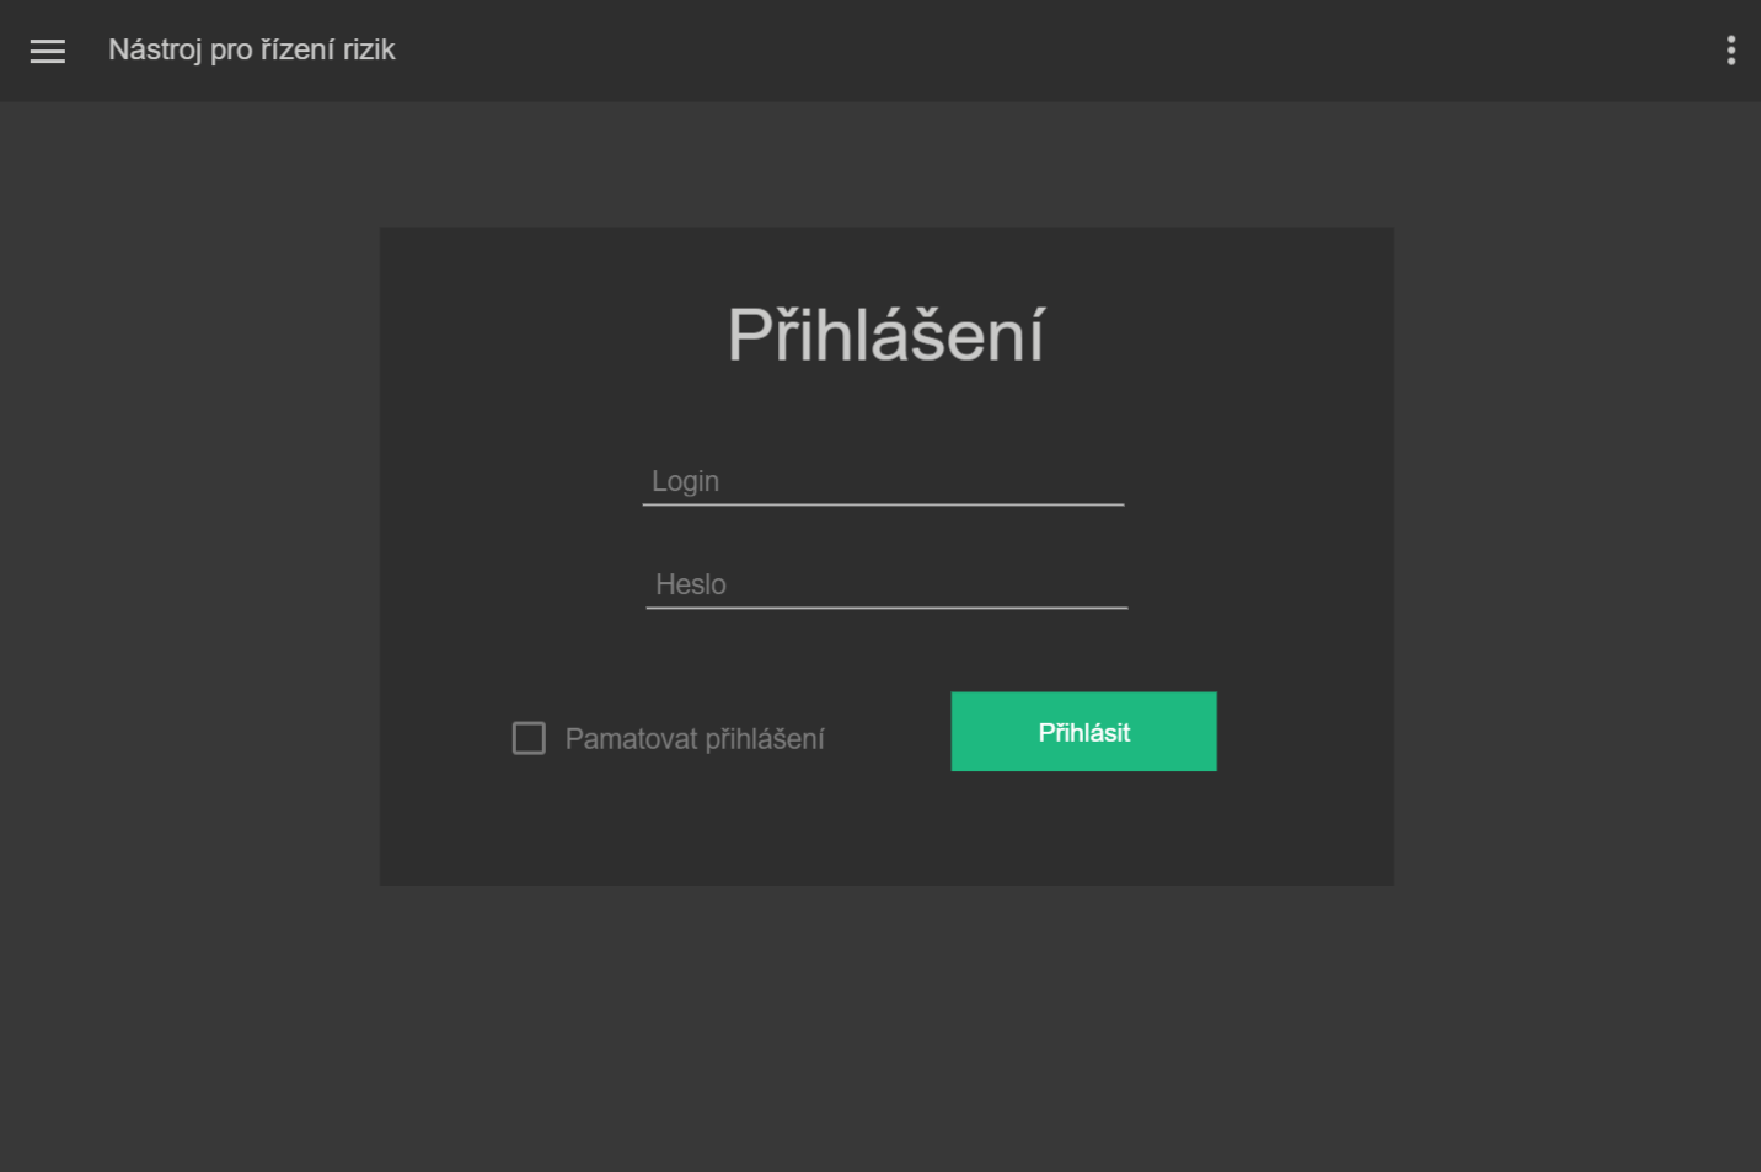
\includegraphics{obrazky-figures/Prihlaseni.pdf}}
    \caption{Návrh přihlašovácí stránky [zdroj vlastní]}
    \label{guiPrihlaseni}
    \end{center}
    \end{figure}
    
    \begin{figure}[!h]
    \begin{center}
    \scalebox{0.5}{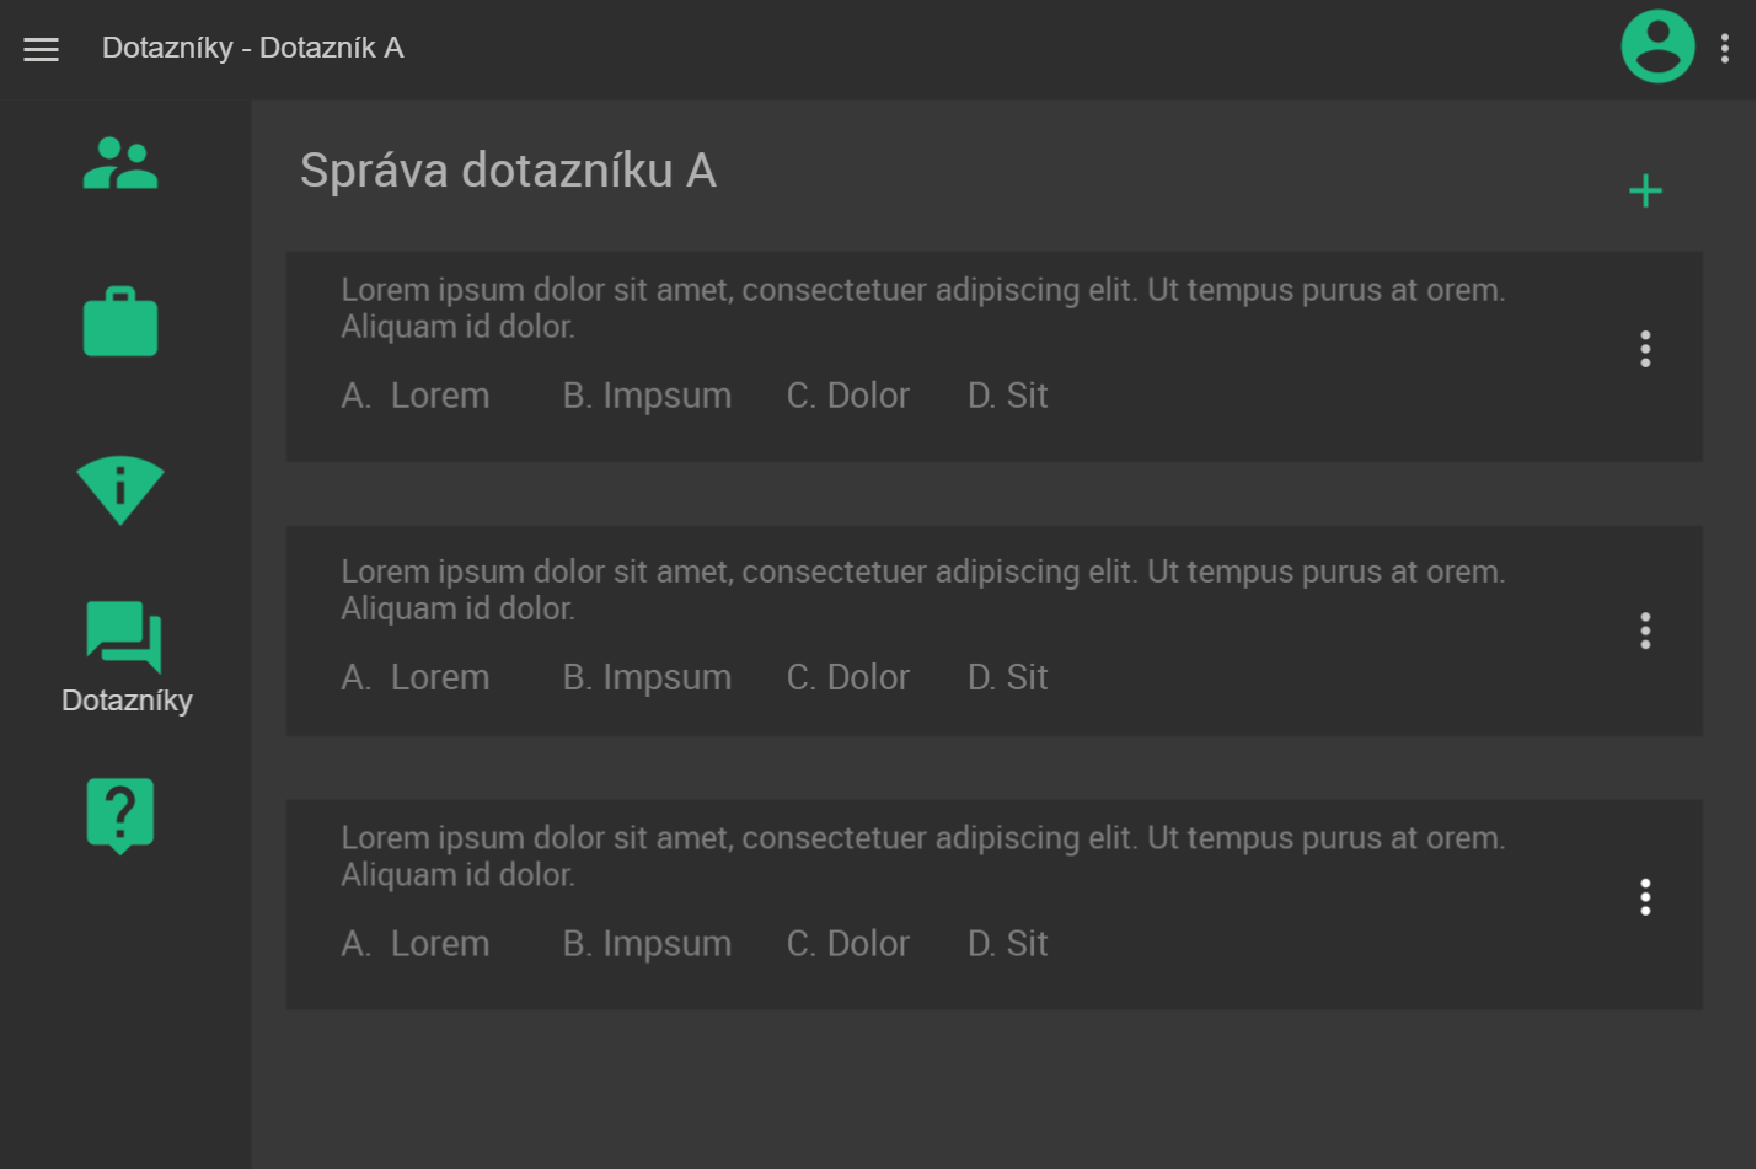
\includegraphics{obrazky-figures/SpravaDotaz.pdf}}
    \caption{Návrh stránky správy dotazníku [zdroj vlastní]}
    \label{guiDotaz}
    \end{center}
    \end{figure}

\chapter{API serveru}
\label{prilohaApi}

Všechna URI mají předponu \texttt{api/nprr}.

\section{RoleController}
\begin{DESCRIPTION}
    \item \texttt{\textbf{POST /role}} Tvorba/editace role.
    \item \texttt{\textbf{GET /secRoles}} Získání všech bezpečnostních rolí.
    \item \texttt{\textbf{GET /secRole/{id}}} Získání bezpečnostní role dle jejího id.
    \item \texttt{\textbf{GET /roles}} Získání všech rolí.
     \item \texttt{\textbf{GET /role}} Získání role aktualně přihlašeného uživatele.
    \item \texttt{\textbf{GET /role/{id}}} Získání role dle jejího id.
    \item \texttt{\textbf{DELETE /role/{id}}} Smazání role dle jejího id.
\end{DESCRIPTION}

\section{UzivatelController}
\begin{DESCRIPTION}
\item \texttt{\textbf{POST /user}} Tvorba/editace uživatele.
\item \texttt{\textbf{GET /users}} Získání všech uživatelů.
\item \texttt{\textbf{GET /info}} Získání informací o~aktuálně přihlašeném uživateli.
\item \texttt{\textbf{GET /users/count}} Počet záznamů v~tabulce s~uživateli.
\item \texttt{\textbf{GET /user/{id}}} Získání uživatele dle jeho id.
\item \texttt{\textbf{GET /user}} Získání všech dat o~aktualně přihlašeném uživateli.
\item \texttt{\textbf{DELETE /user/{id}}} Smazání uživatele dle jeho id.
\end{DESCRIPTION}

\section{KategorieController}
\begin{DESCRIPTION}
\item \texttt{\textbf{POST /kategorie}} Tvorba/editace kategorie rizika.
\item \texttt{\textbf{GET /kategories}} Získání všech kategorií rizik.
\item \texttt{\textbf{GET /kategorie/{id}}} Získání kategorie rizika dle jejího id.
\item \texttt{\textbf{DELETE /kategorie/{id}}} Smazání kategorie rizika dle jejího id.
\end{DESCRIPTION}

\section{RegistrRizikController}
\begin{DESCRIPTION}
\item \texttt{\textbf{POST /risk}} Tvorba/editace rizika v~centrálním registru.
\item \texttt{\textbf{GET /risks}} Získání všech rizik z~centralního registru.
\item \texttt{\textbf{GET /risks/count}} Počet záznamů v~tabulce centralního registru rizik.
\item \texttt{\textbf{GET /risk/{id}}} Získání rizika dle jeho id.
\item \texttt{\textbf{DELETE /risk/{id}}} Smazání rizika dle jeho id.
\end{DESCRIPTION}

\section{OblastOtazkyController}
\begin{DESCRIPTION}
\item \texttt{\textbf{POST /questionArea}} Tvorba/editace oblasti otázky.
\item \texttt{\textbf{GET /questionAreas}} Získání všech oblastí.
\item \texttt{\textbf{GET /questionArea/{id}}} Získání oblasti otázky dle jejího id.
\item \texttt{\textbf{DELETE /questionArea/{id}}} Smazání oblasti otázky dle jejího id.
\end{DESCRIPTION}

\section{OdpovedController}
\begin{DESCRIPTION}
\item \texttt{\textbf{POST /answer}} Tvorba/editace oblasti otázky.
\item \texttt{\textbf{GET /answers}} Získání všech oblastí.
\item \texttt{\textbf{GET /answer/{id}}} Získání oblasti otázky dle jejího id.
\item \texttt{\textbf{DELETE /questionArea/{id}}} Smazání oblasti otázky dle jejího id.
\end{DESCRIPTION}

\section{OtazkaController}
\begin{DESCRIPTION}
\item \texttt{\textbf{POST /question}} Tvorba/editace otázky.
\item \texttt{\textbf{GET /questions}} Získání všech otázek.
\item \texttt{\textbf{GET /question/{id}}} Získání otázky dle jejího id.
\item \texttt{\textbf{DELETE /question/{id}}} Smazání otázky dle jejího id.
\end{DESCRIPTION}

\section{DotaznikController}
\begin{DESCRIPTION}
\item \texttt{\textbf{POST /survey}} Tvorba/editace dotazníku.
\item \texttt{\textbf{GET /surveys}} Získání všech dotazníků.
\item \texttt{\textbf{GET /surveys/cards}} Vrátí objekty karet dotazníků, které shnují jeho základní informace.
\item \texttt{\textbf{GET /survey/{id}}} Získání dotazníku dle jeho id.
\item \texttt{\textbf{DELETE /survey/{id}}} Smazání dotazníku dle jeho id.
\end{DESCRIPTION}

\section{ProjektController}
\begin{DESCRIPTION}
\item \texttt{\textbf{POST /project}} Tvorba/editace projektu - základní informace.
\item \texttt{\textbf{POST /project/survey}} Přiřazení dotazníku ke projektu.
\item \texttt{\textbf{POST /project/{idProj}/survey/{idSurv}/user/{idUser}}} Uložení do databáze informaci o~tom, jak uživatel odpověděl na daný dotazník na projektu.
\item \texttt{\textbf{POST /project/swot}} Tvorba/editace SWOT tabulky projektu.
\item \texttt{\textbf{POST /project/{id}/manager}} Přidání/změna manažera projektu.
\item \texttt{\textbf{POST /project/{id}/users}} Přidání/změna ostatních řešitelů projektu.
\item \texttt{\textbf{POST /project/{id}/risk}} Přiřazení rizika k~projektu.
\item \texttt{\textbf{GET /projects/active/user}} Získání modifikovaných objektů aktivních projektů, na kterých pracuje aktuálně přihlášený uživatel. 
\item \texttt{\textbf{GET /projects/active/{isActive}/manager}} Získání modifikovaných objektů aktivních či neaktivních projektů, na kterých pracuje akutalně přihlášený manažer. 
\item \texttt{\textbf{GET /projects/active/{isActive}}} Získání modifikovaných objektů aktivních či neaktivních projektů.
\item \texttt{\textbf{GET /projects}} Získání všech projektů.
\item \texttt{\textbf{GET /projects/cards}} Získání objektů karet všech projektů, které shrnují jeho základní informace.
\item \texttt{\textbf{GET /projects/cards/user/{id}}} Získání objektů karet všech projektu, které shrnují jeho základní informace. Uživatel s~daným id je aktivním řešitelem nebo manažerem projektu.
\item \texttt{\textbf{GET /project/{id}}} Získání projektu s~daným id.
\item \texttt{\textbf{GET /project/{id}/users}} Získání všech aktivních i neaktivních řešitelů a manažerů projektu.
\item \texttt{\textbf{GET /project/{id}/survey}} Získání dat dotazníků, které se týkají projektu\,--\,jak uživatelé odpovídali na dotazník.
\item \texttt{\textbf{GET /project/{id}/risks}} Získání všech rizik přidělených projektu.
\item \texttt{\textbf{DELETE /project/{id}}} Smazání projektu dle jeho id.
\item \texttt{\textbf{DELETE /project/{id}/swot}} Smazání SWOT tabulky z~projektu dle jeho id.
\item \texttt{\textbf{DELETE /project/{id}/risk/{idRisk}}} Odebrání rizika z~projektu.
\item \texttt{\textbf{DELETE /project/{id}/survey}} Odebrání dotazníku z~projektu.
\end{DESCRIPTION}

\chapter{Příklad dotazníku}
\label{prikladDotazniku}

Vytvořené dotazníky se mohou (podle otázek, které obsahují) zaměřovat na určité oblasti projektu. Příkladem mohou být oblasti rozpočtu projektu, komunikace se zainteresovanými stranami nebo použitých technologií na projektu.

Na následujících řádcích se nachází příklad obecného dotazníků, který obsahuje otázky z~různých oblastí.

\begin{enumerate}
    \item Rozumíte plně používaným technologiím? 
    \begin{itemize}
        \item Ano
        \item Ne
        \item Možná
        \item Nevím
    \end{itemize}
    \item Je zadavatel obeznámen s~riziky na projektu? 
        \begin{itemize}
        \item Ano
        \item Ne
    \end{itemize}
    \item Myslíte si, že projekt je dostatečně financován? 
     \begin{itemize}
        \item Ano
        \item Ne
        \item Nevím
    \end{itemize}
    \item Bylo na identifikaci a analýzu rizik dostatečně času? 
     \begin{itemize}
        \item Ano
        \item Ne
    \end{itemize}
    \item Je cílový uživatel dostatečně zapojen do vývoje projektu? 
       \begin{itemize}
        \item Ano
        \item Ne
    \end{itemize}
    \item Byla alespoň nějaká část vyvíjeného programu představena zákazníkovi? 
            \begin{itemize}
        \item Ano
        \item Ne
    \end{itemize}
\end{enumerate}

\chapter{Testovací scénáře použitelnosti aplikace}
\label{testPodrobnosti}
\begin{enumerate}
    \item Firma přijala dva nové zaměstnance\,--\,Alana Rigera na pozici projektového manažera a Betty Rocky jako členku řešitelského týmu. Je nutné jim vytvořit účet, aby mohli aplikaci využívat. Tuto akci může provádět pouze administrátor.
    \item Firma získala zakázku na nový projekt se zaměřením na záchranu velkých kočkovitých šelem. Jako administrátor je tvou povinností tento projekt vytvořit v~nástroji a tím ho uložit do databáze. Název projektu je Kočkovité šelmy a je popsán jako projekt vytvoření informačního systému pro záchrannou stanici velkých kočkovitých šelem. Začátek prací na projektu byl stanoven na 20.5.2020 a konec se předpokládá někdy na druhou polovinu roku 2022. Nově přijatí zaměstnanci (Alan Riger a Betty Rocky) jsou prvními členy řešitelského týmu a jsou přiřazeni ke svým odpovídajícím pozicím.
    \item Pro projekt Kočkovité šelmy je nutné vytvořit nový dotazník, který může pomoct řešitelům projektu identifikovat rizika, která se mohou vyskytnou na tomto projektu. Před tvorbou dotazníku je vhodné zkontrolovat, zda v~nástroji existují požadované otázky, které má dotazník obsahovat.
    \item Jako manažer (Alan Riger) ti byl přiřazen nový projekt, který máš řídit. Projekt má pracovní název Kočkovité šelmy. Nově bylo ustanoveno, že datum ukončení bude 30.9.2022. Zároveň ti bylo sděleno, že Betty Rocky byla přesunuta do jiného projektu a jako náhrada za ní je přidělena Diana Laris. Změň informace na projektu, aby odpovídaly novým skutečnostem.
    \item Řešitelský tým projektu Kočkovité šelmy identifikoval dvě nová rizika. Riziko Překročení rozpočtu z~kategorie Finance je již známé a je již uložené v~centrálním registru rizik. Projekt je ale dobře financován, takže i když má střední pravděpodobnost výskytu, tak bude mít na projekt pouze minimální dopad. Druhé riziko tým identifikoval poprvé – Pandemie infekční nemoci. Z~důvodu situace ve světě je veliká pravděpodobnost, že riziko zastihne i tento projekt, přičemž bude mít nejvyšší úroveň dopadu. Z~tohoto důvodu by riziko mělo mít nejvyšší prioritu dalšího řešení. Jelikož se první riziko týká financí je vhodné, aby ho měl na starost manažer projektu. U~druhého rizika může být správcem kdokoliv.
    \item Jako manažer se chystáš vytvořit SWOT analýzu projektu Kočkovité šelmy. Pro jednodušší práci se můžeš inspirovat jinými projekty v~systému.
    \item Bylo ti oznámeno, že dotazník k~projektu Kočkovité šelmy je připraven. Přiřadit ho k~tomuto projektu, aby ostatní řešitelé mohli na něho odpovídat. Tuto akci proveď jako manažer daného projektu.
    \item Jednou z~povinností řádového člena týmu je zodpovědět dotazník, který byl přiřazený k~projektu, na kterém daný člen pracuje. Ujisti se, že jsi na něho zodpověděl a pokud ne, tak ho zodpověz.
    \item Zajímá tě, jak ostatní uživatelé odpověděli na dotazník. Zjisti si tuto informaci.
    \item Jsi ve tmavé místnosti a bílé pozadí aplikace dráždí tvé oči. Pokus se tento problém v~aplikaci vyřešit.
    \item Dostal jsi za úkol přepsat z~papíru několik rizik do centrálního registru\,--\,proveď to.
    \item Projekt Kočkovité šelmy skončil neúspěchem. Firma nechce uchovávat jeho data. Jako administrátor jsi dostal za úkol tento projekt ze systému odstranit.
\end{enumerate}

\begin{table}[h]
\centering
\begin{tabular}{|l|l|}
\hline
\textbf{Číslo scénáře:} & 1 \\ \hline
\textbf{Oblast:}        & Správa uživatelů, tvorba uživatelského účtu. \\ \hline 
\multirow{2}{*}{\textbf{Vstupní podmínky:}} & 1. Server běží na pozadí, klientská část je načtená v~prohlížeči. \\ \cline{2-2} 
                                            & 2. Uživatel není přihlášený. \\ \hline
\multirow{3}{*}{\textbf{Očekávaný postup:}} & 1. Přihlásit se jako administrátor.\\ \cline{2-2} 
                                            & 2. V~menu kliknout na položku \textit{Uživatelé}.  \\ \cline{2-2} 
                                            & \begin{tabular}[c]{@{}l@{}}3. V~tabulce \textit{Uživatelé} kliknout na ikonové tlačítko s~popiskem \\ \textit{Přidat}, vyplnit požadované položky v~dialogu a stisknutím tlačítka \\\textit{Uložit} odeslat data na server. Zopakovat i pro druhého \\uživatele.\end{tabular} \\ \hline
\textbf{Očekávaný výsledek:} & 1. V~tabulce \textit{Uživatelé} lze najít nově přidané záznamy. \\ \hline
\end{tabular}
\caption{Podrobnosti pro scénář 1}
\end{table}

\begin{table}[h]
\begin{tabular}{|l|l|}
\hline
\textbf{Číslo scénáře:} & 2 \\ \hline
\textbf{Oblast:} & Tvorba nového projektu. \\ \hline
\multirow{3}{*}{\textbf{Vstupní podmínky:}}   & 1. Server běží na pozadí, klientská část je načtená v~prohlížeči. \\ \cline{2-2} 
                                              & 2. Uživatel je přihlášený jako administrátor. \\ \cline{2-2} 
                                              & 3. Byl proveden předcházející scénář.  \\ \hline
\multirow{2}{*}{\textbf{Očekávaný postup:}}   & 1. V~menu kliknout na položku \textit{Projekty}. \\ \cline{2-2} 
                                              & \begin{tabular}[c]{@{}l@{}}2. V~pravém horním rohu kliknout na ikonové tlačítko s~popiskem  \\ \textit{Přidat}, vyplnit požadované položky a stisknutím tlačítka \\ \textit{Odeslat} odeslat data na server.\end{tabular} \\ \hline
\multirow{2}{*}{\textbf{Očekávaný výsledek:}} & \begin{tabular}[c]{@{}l@{}}1. Uživatel je po odeslání dat přesměrován na stránku nově \\ vytvořeného projektu.\end{tabular}    \\ \cline{2-2} 
                                              & 2. Na stránce projektu lze nalézt informace zadané při tvorbě. \\ \hline
\end{tabular}
\caption{Podrobnosti pro scénář 2}
\end{table}

\begin{table}[h]
\begin{tabular}{|l|l|}
\hline
\textbf{Číslo scénáře:}  & 3  \\ \hline
\textbf{Oblast:} & Správa otázek, tvorba otázky, tvorba dotazníku. \\ \hline
\multirow{3}{*}{\textbf{Vstupní podmínky:}}   & 1. Server běží na pozadí, klientská část je načtená v~prohlížeči.  \\ \cline{2-2} 
                                              & 2. Uživatel je přihlášený jako administrátor.  \\ \cline{2-2} 
                                              & 3. Byl proveden předcházející scénář.  \\ \hline
\multirow{7}{*}{\textbf{Očekávaný postup:}}   & 1. V~menu kliknout na položku \textit{Otázky}.  \\ \cline{2-2} 
                                              & \begin{tabular}[c]{@{}l@{}} 2. V~tabulce \textit{Otázky} pomocí vyhledávacího pole vyhledat \\ požadované otázky.\end{tabular} \\ \cline{2-2} 
                                              & \begin{tabular}[c]{@{}l@{}}3. V~tabulce \textit{Otázky} kliknout na ikonové tlačítko s~popiskem \\ \textit{Přidat}, vyplnit požadované položky v~dialogu a stisknutím\\ tlačítka \textit{Uložit} odeslat chybějící otázku na server.\end{tabular} \\ \cline{2-2} 
                                              & 4. V~menu kliknout na položku \textit{Dotazníky}. \\ \cline{2-2} 
                                              & \begin{tabular}[c]{@{}l@{}}5. V~pravém horním rohu kliknout na ikonové tlačítko s~popiskem \\\textit{Přidat} a vyplnit požadované položky.\end{tabular}  \\ \cline{2-2} 
                                              & \begin{tabular}[c]{@{}l@{}}6. Stisknutím ikonového tlačítka s~popiskem \textit{Přidat otázky} vybrat\\ z~dialogu požadované otázky a stisknutím tlačítka \textit{Uložit} je vložit\\ do dotazníku.\end{tabular}   \\ \cline{2-2} 
                                              & \begin{tabular}[c]{@{}l@{}}7. Stisknutím ikonového tlačítka s~popiskem \textit{Potvrdit} uložit\\ dotazník na server.\end{tabular}   \\ \hline
\multirow{3}{*}{\textbf{Očekávaný výsledek:}} & 1. V~tabulce \textit{Otázky} lze najít nově přidanou otázku.  \\ \cline{2-2} 
                                              & \begin{tabular}[c]{@{}l@{}}2. Po odeslání dotazníku je uživatel přesměrován na stránku\\ nově vytvořeného dotazníku.\end{tabular}  \\ \cline{2-2} 
                                              & 3. Na stránce dotazníku lze nalézt informace zadané při tvorbě.   \\ \hline
\end{tabular}
\caption{Podrobnosti pro scénář 3}
\end{table}

\begin{table}[h]
\begin{tabular}{|l|l|}
\hline
\textbf{Číslo scénáře:}  & 4  \\ \hline
\textbf{Oblast:} & Správa projektu, editace základních informací projektu. \\ \hline
\multirow{3}{*}{\textbf{Vstupní podmínky:}} & 1. Server běží na pozadí, klientská část je načtená v~prohlížeči. \\ \cline{2-2} 
                                            & 2. Uživatel je přihlášený jako administrátor. \\ \cline{2-2} 
                                            & 3. Byl proveden předcházející scénář. \\ \hline
\multirow{4}{*}{\textbf{Očekávaný postup:}} & \begin{tabular}[c]{@{}l@{}}1. Odhlásit se z~aplikace a přihlásit se jako Alan Riger\,--\,manažer\\ projektu.\end{tabular}  \\ \cline{2-2} 
                                            & \begin{tabular}[c]{@{}l@{}}2. Na úvodní \textit{Dashboard} stránce kliknout na kartě požadovaného \\ projektu na tlačítko \textit{Přejít k~projektu}.\end{tabular}  \\ \cline{2-2} 
                                            & \begin{tabular}[c]{@{}l@{}}3. Na kartě \textit{Informace o~projektu} změnit požadované informace \\ (\textit{Datumy projektu} a \textit{Řešitelé projektu}) stisknutím ikonového\\ tlačítka s~popiskem \textit{Editovat}.\end{tabular} \\ \cline{2-2} 
                                            & \begin{tabular}[c]{@{}l@{}}4. Stisknutím ikonového tlačítka s~popiskem \textit{Potvrdit} odeslat \\ nová data na server (každá část je samostatně).\end{tabular}\\ \hline
\textbf{Očekávaný výsledek:}                & 1. Na kartě \textit{Informace o~projektu} lze vidět nově zadaná data.\\ \hline
\end{tabular}
\caption{Podrobnosti pro scénář 4}
\end{table}

\begin{table}[]
\begin{tabular}{|l|l|}
\hline
\textbf{Číslo scénáře:} & 5\\ \hline
\textbf{Oblast:} & Správa projektu, přidání nového rizika, přiřazení rizika k~projektu. \\ \hline
\multirow{4}{*}{\textbf{Vstupní podmínky:}}   & 1. Server běží na pozadí, klientská část je načtená v~prohlížeči.   \\ \cline{2-2} 
                                              & 2. Uživatel je přihlášený jako Alan Riger. \\ \cline{2-2} 
                                              & 3. Byl proveden předcházející scénář. \\ \cline{2-2} 
                                              & 4. Uživatel se nachází na stránce požadovaného projektu.\\ \hline
\multirow{3}{*}{\textbf{Očekávaný postup:}}   & 1. Přejít na kartu \textit{Rizika projektu}.\\ \cline{2-2} 
                                              & \begin{tabular}[c]{@{}l@{}}2. V~tabulce \textit{Registr rizik} kliknout na ikonové tlačítko s~popiskem\\ \textit{Přidat}. V~dialogu kliknutím na tlačítko \textit{Centrální registr} načíst\\ rizika z~centrálního registru. Vybrat požadované riziko, doplnit\\ informace a stisknutím tlačítka \textit{Uložit} přidělit riziko k~projektu.\end{tabular} \\ \cline{2-2} 
                                              & \begin{tabular}[c]{@{}l@{}}3. Opět kliknout na ikonové tlačítko s~popiskem \textit{Přidat}. V~dialogu\\ kliknout na tlačítko \textit{Nové riziko} a doplnit informace nového rizika\\ (tvorba rizika). Stisknutím tlačítka \textit{Uložit} přidělit riziko k~projektu\\ a zároveň uložit do centrálního registru.\end{tabular}                   \\ \hline
\multirow{2}{*}{\textbf{Očekávaný výsledek:}} & \begin{tabular}[c]{@{}l@{}}1. Na kartě \textit{Rizika projektu} v~tabulce \textit{Registr rizik} lze vidět \\přiřazená rizika. \textit{Matice pravděpodobností a dopadů} zobrazuje\\ rizika. Grafy zobrazují statistické informace.\end{tabular}\\ \cline{2-2} 
                                              & 2. Nově tvořené riziko se nachází v~\textit{Centrálním registru rizik}. \\ \hline
\end{tabular}
\caption{Podrobnosti pro scénář 5}
\end{table}

\begin{table}[h]
\begin{tabular}{|l|l|}
\hline
\textbf{Číslo scénáře:}  & 6  \\ \hline
\textbf{Oblast:}  & Správa projektu, tvorba SWOT.  \\ \hline
\multirow{4}{*}{\textbf{Vstupní podmínky:}} & 1. Server běží na pozadí, klientská část je načtená v~prohlížeči.\\ \cline{2-2} 
                                            & 2. Uživatel je přihlášený jako Alan Riger.  \\ \cline{2-2} 
                                            & 3. Byl proveden předcházející scénář.    \\ \cline{2-2} 
                                            & 4. Uživatel se nachází na stránce požadovaného projektu. \\ \hline
\multirow{3}{*}{\textbf{Očekávaný postup:}} & 1. Přejít na kartu \textit{SWOT analýza}. \\ \cline{2-2} 
                                            & 2. Kliknout na tlačítko \textit{Přidat SWOT analýzu}.  \\ \cline{2-2} 
                                            & \begin{tabular}[c]{@{}l@{}}3. Vyplnit požadované položky a stisknutím ikonového tlačítka\\ s~popiskem \textit{Potvrdit} uložit data na server.\end{tabular} \\ \hline
\textbf{Očekávaný výsledek:}                & \begin{tabular}[c]{@{}l@{}}1. Na kartě \textit{SWOT analýza} lze vidět vytvořenou swot tabulku\\ v~zobrazovacím režimu.\end{tabular} \\ \hline
\end{tabular}
\caption{Podrobnosti pro scénář 6}
\end{table}

\begin{table}[]
\begin{tabular}{|l|l|}
\hline
\textbf{Číslo scénáře:}  & 7   \\ \hline
\textbf{Oblast:} & Správa projektu, přiřazení dotazníku. \\ \hline
\multirow{4}{*}{\textbf{Vstupní podmínky:}}   & 1. Server běží na pozadí, klientská část je načtená v~prohlížeči. \\ \cline{2-2} 
                                              & 2. Uživatel je přihlášený jako Alan Riger. \\ \cline{2-2} 
                                              & 3. Byl proveden předcházející scénář.  \\ \cline{2-2} 
                                              & 4. Uživatel se nachází na stránce požadovaného projektu.\\ \hline
\multirow{3}{*}{\textbf{Očekávaný postup:}}   & 1. Přejít na kartu \textit{Dotazník}. \\ \cline{2-2} 
                                              & 2. Kliknout na tlačítko \textit{Přidat dotazník}. \\ \cline{2-2} 
                                              & \begin{tabular}[c]{@{}l@{}}3. Ve výběrovém dialogu kliknout na požadovaný dotazník, čímž \\ se zobrazí jeho podrobnosti, a následně kliknutím na tlačítko \\ \textit{Přiřadit} ho přidat k~projektu.\end{tabular} \\ \hline
\multirow{2}{*}{\textbf{Očekávaný výsledek:}} & 1. Na kartě \textit{Dotazník} lze vidět základní informace dotazníku. \\ \cline{2-2} 
                                              & \begin{tabular}[c]{@{}l@{}}2. Zobrazily se tlačítka na zodpovězení, zobrazení statistiky \\ a smazání dotazníku.\end{tabular} \\ \hline
\end{tabular}
\caption{Podrobnosti pro scénář 7}
\end{table}

\begin{table}[h]
\begin{tabular}{|l|l|}
\hline
\textbf{Číslo scénáře:}  & 8  \\ \hline
\textbf{Oblast:}  & Správa projektu, zodpovězení dotazníku. \\ \hline
\multirow{3}{*}{\textbf{Vstupní podmínky:}}   & 1. Server běží na pozadí, klientská část je načtená v~prohlížeči.  \\ \cline{2-2} 
                                              & 2. Uživatel je přihlášený jako Alan Riger.  \\ \cline{2-2} 
                                              & 3. Byl proveden předcházející scénář. \\ \hline
\multirow{5}{*}{\textbf{Očekávaný postup:}}   & \begin{tabular}[c]{@{}l@{}}1. Odhlásit se z~aplikace a přihlásit se jako Diana Laris – člen \\ týmu.\end{tabular} \\ \cline{2-2} 
                                              & \begin{tabular}[c]{@{}l@{}}2. Na úvodní \textit{Dashboard} stránce kliknout na kartě požadovaného \\ projektu na tlačítko \textit{Přejít k~projektu}.\end{tabular} \\ \cline{2-2} 
                                              & 3. Přejít na kartu \textit{Dotazník}. \\ \cline{2-2} 
                                              & \begin{tabular}[c]{@{}l@{}}4. Kliknutím na tlačítko \textit{Zodpovědět} zodpovědět na otázky, které \\ se zobrazily v~dialogu.\end{tabular}  \\ \cline{2-2} 
                                              & \begin{tabular}[c]{@{}l@{}}5. Po zodpovězení všech otázek kliknout na tlačítko \textit{Odeslat}, čímž \\ se odpovědi odešlou na server.\end{tabular} \\ \hline
\multirow{2}{*}{\textbf{Očekávaný výsledek:}} & \begin{tabular}[c]{@{}l@{}}1. Na kartě \textit{Dotazník} se v~části \textit{Zodpovězený dotazník} změní \\ informace, že uživatel zodpověděl na dotazník.\end{tabular} \\ \cline{2-2} 
                                              & 2. Tlačítko \textit{Výsledky} je viditelné.  \\ \hline
\end{tabular}
\caption{Podrobnosti pro scénář 8}
\end{table}

\begin{table}[h]
\begin{tabular}{|l|l|}
\hline
\textbf{Číslo scénáře:} & 9  \\ \hline
\textbf{Oblast:}  & Správa projektu, zobrazení statistiky dotazníku. \\ \hline
\multirow{4}{*}{\textbf{Vstupní podmínky:}} & 1. Server běží na pozadí, klientská část je načtená v~prohlížeči. \\ \cline{2-2} 
                                            & 2. Uživatel je přihlášený jako Diana Laris.  \\ \cline{2-2} 
                                            & 3. Byl proveden předcházející scénář.  \\ \cline{2-2} 
                                            & 4. Uživatel se nachází na stránce požadovaného projektu.  \\ \hline
\multirow{2}{*}{\textbf{Očekávaný postup:}} & 1. Přejít na kartu \textit{Dotazník}. \\ \cline{2-2} 
                                            & 2. Kliknutím na tlačítko \textit{Výsledky} zobrazit statistiku. \\ \hline
\textbf{Očekávaný výsledek:}                & \begin{tabular}[c]{@{}l@{}}1. Na kartě \textit{Dotazník} je zobrazena celková statistika, jak zodpovědní \\ uživatelé odpovídali na dotazník.\end{tabular} \\ \hline
\end{tabular}
\caption{Podrobnosti pro scénář 9}
\end{table}

\begin{table}[h]
\begin{tabular}{|l|l|}
\hline
\textbf{Číslo scénáře:}  & 10 \\ \hline
\textbf{Oblast:}   & Přepnutí do tmavého režimu. \\ \hline
\multirow{2}{*}{\textbf{Vstupní podmínky:}} & 1. Server běží na pozadí, klientská část je načtená v~prohlížeči.  \\ \cline{2-2} 
                                            & 2. Uživatel je přihlášený. \\ \hline
\textbf{Očekávaný postup:} & \begin{tabular}[c]{@{}l@{}}1. V~hlavním aplikačním rámci kliknout na ikonové tlačítko \\ s~popiskem \textit{Tmavý režim}.\end{tabular} \\ \hline
\textbf{Očekávaný výsledek:} & 1. Aplikace se nachází v~tmavém režimu. \\ \hline
\end{tabular}
\caption{Podrobnosti pro scénář 10}
\end{table}

\begin{table}[h]
\begin{tabular}{|l|l|}
\hline
\textbf{Číslo scénáře:}  & 11 \\ \hline
\textbf{Oblast:} & Správa centrálního registru rizik, tvorba nového rizika.\\ \hline
\multirow{2}{*}{\textbf{Vstupní podmínky:}} & 1. Server běží na pozadí, klientská část je načtená v~prohlížeči. \\ \cline{2-2} 
                                            & 2. Uživatel je přihlášený.  \\ \hline
\multirow{2}{*}{\textbf{Očekávaný postup:}} & 1. V~menu kliknout na položku \textit{Registr rizik}.\\ \cline{2-2} 
                                            & \begin{tabular}[c]{@{}l@{}}2. V~tabulce \textit{Registr rizik} kliknout na ikonové tlačítko s~popiskem\\ \textit{Přidat}, vyplnit požadované položky v~dialogu a stisknutím tlačítka\\ \textit{Uložit} odeslat data na server. V~případě potřeby zopakovat.\end{tabular} \\ \hline
\textbf{Očekávaný výsledek:}                & 1. V~tabulce \textit{Registr rizik} lze nalézt nově přidané záznamy. \\ \hline
\end{tabular}
\caption{Podrobnosti pro scénář 11}
\end{table}

\begin{table}[h]
\begin{tabular}{|l|l|}
\hline
\textbf{Číslo scénáře:} & 12 \\ \hline
\textbf{Oblast:}  & Správa projektu, smazání projektu.\\ \hline
\multirow{3}{*}{\textbf{Vstupní podmínky:}}   & 1. Server běží na pozadí, klientská část je načtená v~prohlížeči.  \\ \cline{2-2} 
                                              & 2. Uživatel je přihlášený jako administrátor.\\ \cline{2-2} 
                                              & 3. Byl proveden scénář 10. \\ \hline
\multirow{3}{*}{\textbf{Očekávaný postup:}}   & 1. V~menu kliknout na položku \textit{Projekty}.  \\ \cline{2-2} 
                                              & 2. V~kartě požadovaného projektu kliknout na tlačítko \textit{Smazat}. \\ \cline{2-2} 
                                              & 3. V~potvrzovacím dialogu kliknout na tlačítko \textit{Potvrdit}.  \\ \hline
\multirow{2}{*}{\textbf{Očekávaný výsledek:}} & 1. V~přehledu projektů se nenachází karta smazaného projektu \\ \cline{2-2} 
                                              & \begin{tabular}[c]{@{}l@{}}2. Pokus o~přístup na adresu projektu skončí chybovým \\ hlášením 404.\end{tabular} \\ \hline
\end{tabular}
\caption{Podrobnosti pro scénář 12}
\end{table}

\chapter{Použité knihovny při tvorbě klientské části}
\label{prilohaKnihovny}

Tento seznam, včetně verzí daných knihoven, lze najít v~souboru \texttt{package.json}.

\begin{DESCRIPTION}
\item \texttt{\textbf{date-fns, date-io/date-fns}} Date-fns zpřístupňuje metody pro manipulaci s~kalendářními daty. Date-io/date-fns pak tyto metody abstrahuje a díky tomu je můžou používat i~jiné knihovny.
\item \texttt{\textbf{material-ui/core, material-ui/icons, material-ui/lab, material-ui/pickers}} \newline Jedná se o~různé části z~knihovny Material-UI. Core zpřístupňuje všechny komponenty, které tato knihovna obsahuje. Z~icons se pak přidávají Material Design ikony od společnosti Google. Lab obsahuje komponenty, které jsou ještě ve fázi testování a z~tohoto důvodu ještě nejsou součásti balíčku core. Pickers se používají jako komponenty kalendáře a hodin.
\item \texttt{\textbf{nivo/bar, nivo/heatmap, nivo/pie }} Grafové komponenty z~knihovny Nivo. Nivo umožňuje stáhnout každý graf jako samostatnou knihovnu, aby výsledný balíček byl co nejmenší. Bar představuje sloupcový graf, pie je koláčovým grafem a modifikovaný heatmap se používá pro zobrazení matice pravděpodobnosti a dopadu. 
\item \texttt{\textbf{axios}} Knihovna, která hlavně umožňuje tvořit, posílat a přijímat HTTP požadavky.
\item \texttt{\textbf{formik}} Podpůrná knihovna pro jednodušší správu formulářů. Pro validaci používá knihovnu yup
\item \texttt{\textbf{yup}} Knihovna používá pro validaci dat v~nástroji. Lze použít pro validaci formulářů nebo i samostatných dat.
\item \texttt{\textbf{material-table}} Tato knihovna tvoří komponenty tabulek, které jsou vytvořené ve stylu Material Desing. Vnitřně používá komponenty z~Material-UI
\item \texttt{\textbf{randomcolor}} Knihovna pro vygenerování náhodných barev. Používá se pro vybarvení grafů.
\item \texttt{\textbf{react, react-dom}} Jsou to balíčky z~knihovny React. Obsahují všechny potřebné komponenty pro vytvoření React aplikace. 
\item \texttt{\textbf{react-scripts}} Jde o~balíček skriptů a konfiguračních souborů, které používá Create React App. Create React App se používá pro rychlé a automatické vytvoření výchozí React aplikace.
\item \texttt{\textbf{react-draggable}} Tvoří komponentu, díky které lze její potomky tzv. uchopit a přenášet. Používá se u~některých dialogů.
\item \texttt{\textbf{redux, react-redux}} Redux umožňuje vytvářet a~spravovat globální stav aplikace, react-redux pak zpřístupňuje propojení mezi Reactem a Reduxem. 
\item \texttt{\textbf{redux-auth-wrapper}} Tato knihovna umožňuje definovat přístup k~jednotlivým částem aplikace podle role a oprávnění uživatele. Podobně pak omezuje přístup a viditelnost komponent. Není součástí systému Redux, ale využívá informace uložené v~globálním stavu. 
\item \texttt{\textbf{react-router-dom}} Propojuje DOM s~komponenty knihovny React Router. Díky tomuto lze v~aplikaci provádět směrování. 
\item \texttt{\textbf{react-promise-tracker}} Je to knihovna, která se používá pro sledovaní slibů (\textit{promise}) v~aplikaci. Díky tomuto je možné zobrazovat načítací obrázek v~době, kdy se načítají data ze serveru.
\item \texttt{\textbf{react-swipeable-views}} Knihovna zpřístupňující komponentu pro plynulejší posouvání mezi stránkami na stejné úrovni. Je použita při odpovídání na dotazník projektu.
\end{DESCRIPTION}

\chapter{Návod ke zprovoznění aplikace}
\label{prilohaNavod}

Všechny příkazy, pro jednodušší kopírování, lze také najít v~souboru README. Předpokládá se spuštění na systému Windows 10 či nějakém ekvivalentním operačním systému.

\section{Server}

Server potřebuje pro svůj běh mít nainstalovanou Javu. Serverová část byla primárně tvořena na verzi 1.8.0\_231. Java se musí nacházet v~PATH proměnné.

\begin{enumerate}
    \item V~příkazovém řádku najít zdrojový adresář serveru\,--\,adresář \textbf{server}.
    \item Překlad a vytvoření jar souboru
        \begin{enumerate}
            \item Překlad a spuštění automatizovaných testů před vytvořením jar souboru:
            \begin{verbatim}
                mvnw.cmd clean package
            \end{verbatim}
            \item Vytvoření jar souboru bez překladu testů:
            \begin{verbatim}
                mvnw.cmd -Dmaven.test.skip clean package
            \end{verbatim}
            \item Překlad zdrojových souborů i testů, ale přeskočení spuštění testů před vytvořením jar souboru aplikace:
            \begin{verbatim}
                mvnw.cmd -DskipTests clean package
            \end{verbatim}
        \end{enumerate}
    \item Jar soubor aplikace se nachází v~adresáři target pod názvem \textbf{spravarizik-1.0.jar}. Spuštěná aplikace poběží na \textbf{localhost:8080}. Ze zdrojového adresáře lze spustit s: 
    \begin{verbatim} java -Dfile.encoding=UTF-8 -jar target\spravarizik-1.0.jar \end{verbatim}
    \item Ukončení aplikace: \texttt{ctrl + c}.
    
\end{enumerate}

\section{Klient}

Pro běh klienta na lokálním stoji je nutné mít nainstalovaný Node.js, ten v~sobě již obsahuje správce balíčku npm, který je potřeba pro stažení závislostí a spuštění klienta. Klientská část byla primárně tvořena na node ve verzi 12.15.0 s~npm ve verzi 6.13.7.

\begin{enumerate}
    \item V~příkazovém řádku najít zdrojový adresář klientské části \,--\,adresář \textbf{klient}.
    \item Stažení potřebných závislostí: \texttt{npm i}.
    \item Spuštěná aplikace poběží v~prohlížeči na adrese \textbf{localhost:3000}. Je vhodné zde zmínit, že klient očekává, že server poběží na portu 8080 a podobně server očekává klientskou část na portu 3000. Spustit ji lze pomocí: \texttt{npm start}.
    \item Vytvoření balíčku, které lze následně nahrát na nějaký webový serve: \texttt{npm build}.
    \item Ukončení aplikace: po stisknutí \texttt{ctrl + c} se zobrazí nabídka k~ukončení.
\end{enumerate}

\section{Přihlašovací údaje}

\begin{table}[h]
\centering
\begin{tabular}{|l|l|l|l|}
\hline
ROLE          & LOGIN    & HESLO & JMÉNO         \\ \hline
Administrátor & xlogin00 & qwe   & Login Login   \\ \hline
Manažer       & xriger00 & abc   & Alan Riger    \\ \hline
Manažer       & xhodso00 & abc   & Bianca Hodson \\ \hline
Člen týmu     & xlaris00 & 123   & Diana Laris   \\ \hline
Člen týmu     & xnovak00 & 123   & Casper Novak  \\ \hline
\end{tabular}
\caption{Přihlašovací údaje pro vytvořené účty}
\end{table}

\chapter{Obsah paměťového média}
\label{prilohaCD}

\begin{itemize}
    \item \texttt{README} - Základní popis včetně návodu na zprovoznění aplikace
    \item \texttt{source} - adresář se zdrojovými kódy
    \item \texttt{source/client} - adresář se zdrojovými kódy klientské části
    \item \texttt{source/server} - adresář se zdrojovými kódy serverové části
    \item \texttt{xskuto00.pdf} - tento dokument
    \item \texttt{latex} - adresář se zdrojovými \LaTeX{} soubory tohoto dokumentu
\end{itemize}